\documentclass[a4paper,10pt]{scrartcl}
\usepackage[utf8]{inputenc}
\usepackage[hyphens]{url}
\usepackage{hyperref}
\usepackage[ngerman]{babel}
\usepackage[T1]{fontenc}
\usepackage{graphicx}
\usepackage[utf8]{inputenc}
\usepackage{lmodern}
\usepackage{geometry}
\usepackage{pgfplots} 
\usepackage{mathrsfs}
\usepackage{mathtools}
\usepackage{listings}
\usepackage{wrapfig}
\usepackage{float}
\usepackage{amsmath}
\usepackage{stmaryrd}
\usepackage{paralist}
\lstset{basicstyle=\normalfont\ttfamily,breaklines=true}


\geometry{paper=a4paper, left=25mm, right=25mm, top=35mm, bottom=35mm}
\hypersetup{
    unicode=false,
    pdftoolbar=true,
    pdfmenubar=true,
    pdffitwindow=false,
    pdfstartview={FitH},
    pdftitle={DataScienceReport},
    pdfauthor={PaSeDa},
    pdfsubject={Subject},
    pdfcreator={Creator},
    pdfproducer={Producer},
    pdfkeywords={keyword1} {key2} {key3},
    pdfnewwindow=true,
    colorlinks=false,
    linkcolor=red,
    citecolor=green,
    filecolor=magenta,
    urlcolor=cyan
}

\title{\vspace{2cm} DataScience 1 }
\subtitle{\vspace{4cm}Verbindung von Einkommen  und Wahlverhalten in Frankfurt}
\author{\vspace{5cm}PaSeDa}
\date{}

\usepackage{etoolbox}


%Mathepakete
\usepackage{amsfonts}
\usepackage{amsmath}
\usepackage{amssymb}
\usepackage{amsthm}    

\newcommand{\TODO}{\textcolor{red}{\textbf{TODO }}}

\allowdisplaybreaks
 \pgfplotsset{compat=1.17}
\begin{document}
\maketitle
\newpage
\begin{abstract}
In dieser Arbeit beschreiben wir unser Vorgehen bei der uns in der Vorlesung  "Data Science 1"  im Sommersemester 2020 gestellten Aufgabe. Unsere Aufgabe bestand darin, zwei öffentlich verfügbare Datensätze nach Standards der Data Science zu bearbeiten und zwei unterschiedliche Machine Learning Algorithmen auf diese an zu wenden und diese beiden Algorithmen zu vergleichen.\\
Wir entschieden uns für zwei Datensätze der Stadt Frankfurt. Der erste Datensatz bestand aus Arbeitsmarktdaten nach Stadtteilen gegliedert, der zweite enthielt die Ergebnisse der Bundestagswahl 2017, ebenfalls nach Stadtteilen gegliedert. Die beiden Algorithmen, die wir untersuchen werden, sind \lstinline|GradientBoostingRegressor| und \lstinline|RandomForestRegressor|. \\
\end{abstract}
\newpage
\tableofcontents
.
\newpage
\section{Unsere Infrastruktur}
Unser gesamtes Projekt ist auf \href{Github}{\lstinline|https://github.com/5yntek/DataScienceProject|} zu finden. Die verwendeten Rohdaten sind unter \lstinline|/data| gesammelt. Für die erste Sichtung der Daten verwendeten wir die mit Panda Profiling erstellten Reporte im html Format, die finale Implementierung befindet sich in dem Jupyter Notebook "project patrick". Sämtlicher Code ist Python3. Nennenswerte Bibliotheken, die wir verwendet haben sind \href{https://www.scipy.org/}{scipy} (\href{https://numpy.org/}{numpy}, \href{https://pandas.pydata.org/}{pandas}, \href{https://matplotlib.org/}{matplotlib}), \href{https://scikit-learn.org/}{sklearn}, \href{https://seaborn.pydata.org/}{seaborn}  und \href{https://github.com/pandas-profiling/pandas-profiling}{pandas-profiling}.


\section{Die Daten}
Die verwendetet Arbeitsmarktdaten sind von \href{https://offenedaten.frankfurt.de/dataset/arbeitsmarkt}{Arbeitsmarkt} auf dem Portal \href{https://offenedaten.frankfurt.de} {offenedaten.frankfurt.de} und  nach eigenen Angaben Daten aus dem Jahr 2011 und 2012. Leider ist die auf der Seite angegebene Quelle veraltet, sodass wir die Daten nicht weiter verifizieren konnten, doch da die Daten von der Stadt Frankfurt bereitgestellt werden, nehmen wir an, sie sind korrekt. Dass die Daten nicht aktueller sind ist zwar Schade, sollte für unser Projekt aber kein Hindernis sein. Daten aus zum Beispiel dem statistischen Bundesamt waren für unser Projekt leider nicht passend. 

Mehr Daten werden über Wahlergebnisse erhoben. Alleine auf offenedaten.frankfurt gibt es diverse Datensätze zu verschiedenen Wahlen. Für uns am interessantesten erscheinen Daten zur Bundestagswahl, sodass wir uns für den Datensatz der \href{https://offenedaten.frankfurt.de/dataset/bundestagswahl-2017-ergebnisse-in-frankfurt-am-main}{Bundestagswahl 2017} (im weiteren BW17 genannt) entschieden haben.



\section{Preprocessing}
Bei dem ersten Studium der Daten fielen uns einige fehlenden Datensätze auf. Auch sind die Namen der Stadtteile der beiden Datensätze nicht vollständig identisch.

\subsection{Merge and clean the data}
Dieser Arbeitsschritt ist im Jupyternotebook "data analysis" nach zu vollziehen.\\
Zunächst verwarfen wir Informationen aus den Rohdaten die wir nicht gebrauchen konnten , so zum Beispiel totale Werte. Die Gesamtanzahl der Wähler einer Partei war für uns nicht interessant, da wir nur relative Werte gebrauche konnten, um Stadtteile miteinander vergleichen zu können. Weiterhin sorgten wir dafür, dass numerische Werte richtig interpretiert wurden. Die deutsche Variante der Darstellung von Zahlen ist untypisch und mussten transformiert werden. Einige Sonderzeichen befanden sich in den Bezeichnern der Attribute, die entfernt werden mussten. Die Attributnamen sind generell unpraktisch lang und wurden umbenannt. Die Stadtteile Gutleut- und Bahnhofsviertel wurden in BW17 unter \emph{Gutleut-/Bahnhofsviertel} zusammengefasst und wurden getrennt. Die Anteile des Bruttoarbeitsentgelts waren nicht direkt vorhanden und wurden zunächst aus den anderen Daten errechnet.\\
Nach diesen Schritten führten wir die beiden Tabellen zusammen.


\subsection{pandas-profiling}
Unser nächster Schritt war eine statistische Analyse der Daten. Ein hierfür nützliches Tool ist pandas-profiling. Dieses Framework erzeugt mit wenigen Zeilen einen ausführlichen Bericht in Form von einem HTML-Dokument. Pandas-profiling zeigt unter anderem fehlende Werte, Datentypen und -Bereiche, sowie Korrelation an. Letztere ist besonders interessant. Pandas-profling liefert mehrere gut lesbare Diagramme zu Korrelationen innerhalb der Daten. Ein davon stellt die Pearson-Korrelation (r) da. Diese ist ein Maß für die lineare Korrelation zwischen zwei Variablen. Sein Wert liegt zwischen -1 und +1. -1 steht für maximale negative lineare Korrelation, 0 zeigt keine lineare Korrelation an und 1 zeigt maximale positive lineare Korrelation. Abbildung \ref{fig:correlation}\begin{figure}
	\centering
	\fbox{	
		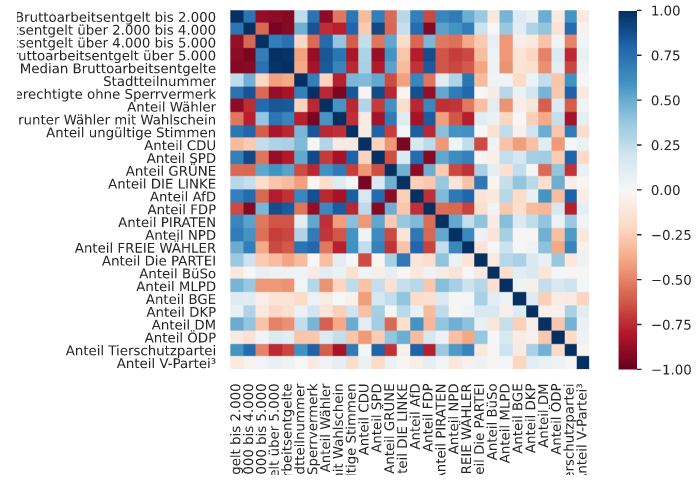
\includegraphics[width=0.8\textwidth]{figure/correlation}
	}
	\caption{Pearson-Korrelation der Daten}
	\label{fig:correlation}
\end{figure}
 stellt die Pearson-Korrelation der Daten da.\\
 Wir diskutierten anhand der verschiedenen Korrelationstabellen aus den drei unterschiedlichen Reporten verschieden Daten, die wir zur Vorhersage verwenden wollten. In die nähere Auswahl fielen schließlich die Daten zum Einkommen und eventuell noch Daten zur Arbeitslosigkeit und Nebenjobdichte. Nach einigen weiteren Untersuchungen dieser Datensätze (zu finden im Ordner "regression", r2 Werte, mögliche lineare Korrelation etc.) auf mögliche Korrelationen dieser Datensätzen zu dem Wahlergebnissen entschieden wir uns für die Einkommensdaten, gegliedert nach Gehaltsgruppen und dem Median (zu finden im "report other").\\     
 
\section{Zielsetzung}
Wir definierten unser Ziel darin, heraus zu finden, ob die beiden unterschiedlichen Algorithmen für eine Prognose des Wahlverhaltens zur Bundestagswahl 2017 in den einzelnen Stadtteilen anhand der Einkommensdaten der Stadtteile in Frankfurt geeignet wären. 

\subsection{Test and verify your data quality}
Im Zusammenhang mit Daten-Qualität existieren unterschiedliche Kriterien. Wichtige sind unter andere Accuray, Relevancy, Completeness, Timliness und Consistency (\href{https://towardsdatascience.com/7-steps-to-ensure-and-sustain-data-quality-3c0040591366}{source}).
\begin{description}
\item[Accuray] Die Daten wurden von der Stadt Frankfurt erhoben und sind damit so akkurat wie möglich. Bei dem mergen der Daten, haben wir sichergestellt, die Bedeutung der Daten nicht zu verändern.
\item[Relevancy] Die von uns verwendeten Daten zu dem Einkommen sind selbstverständlich untereinander korreliert. Nach einigen Untersuchungen mit lediglich dem Median des Einkommens als Datensatz, die zu einer schlechteren Prognose des Wahlverhaltens führten, gehen wir davon aus, dass auch die Einkommensverteilung eine Rolle spielen könnte. Daher erscheinen uns unsere Datenpunkte relevant.
\item[Completness] Die verwendeten Daten sind nach unsere Bearbeitung bis auf zwei Datensätze in allen Punkten komplett. 
\item[Timliness] Für eine realistischere Prognose aktueller Wahlen wären sicherlich aktuellere Einkommensdaten sinnvoll. Doch da wir vermuten, dass sich die Einkommensdaten nicht innerhalb weniger Jahre dramatisch ändern und unsere Aufgabe ebenfalls nicht in der Findung eines möglichst guten Vorhersage Modells besteht, sondern wir hier das Vorgehen im Bereich der Data Science darstellen wollen, sind die Daten für unsere Zwecke geeignet.\\
\item[Consitency] Unsere Daten verwenden überall die selben Datentypen und dieselbe Maßeinheiten. Euro für die Angaben des Einkommen und Prozentangaben für das Wahlergebnis. Sie sind in allen Punkten konsistent.
\end{description}


\subsection{Further preprocessing}
Die eben erwähnten Datenpunkte mit fehlenden Werten wurden entfernt.


\section{Apply two different algorithms of the same kind}
Wir trainierten zwei ML-Modelle, die Vorhersagen über die Verteilung der Wahlstimmen in Abhängigkeit zu der Einkommensverteilung eines Stadtteils treffen.\\
Unsere Target-Values sind Anteil an den Gesamtstimmen in Prozent. Das heißt wir wollen Werte von 0 bis 100 für jede Partei als Ergebnis unserer Vorhersage. Um ein solches Problem zu lösen, bietet sich Multi-Target-Regression an. scikit-learn stellt solche Funktionalität u.a. mit der Klasse \href{https://scikit-learn.org/stable/modules/generated/sklearn.multioutput.MultiOutputRegressor.html}{MultiOutputRegressor} zur Verfügung. Mit ihr ist es leicht gängige scikit-learn Regressionsmodelle für Multi-Target Probleme zu erweitern. Zwei der von uns getesteten Modelle sind \lstinline|GradientBoostingRegressor| und \lstinline|RandomForestRegressor|.
\begin{description}
	\item[GradientBoosting] baut ein additives Modell schrittweise auf. Es ermöglicht die Optimierung beliebig differenzierbarer Verlustfunktionen. In jeder Stufe wird ein Regressionsbaum an den negativen Gradienten der gegebenen Verlustfunktion angepasst
	\item[RandomForest] ist ein Meta-Schätzer, der eine Reihe von klassifizierenden Entscheidungsbäumen für verschiedene Teilstichproben des Datensatzes anpasst und mithilfe der Mittelwertbildung die Vorhersagegenauigkeit verbessert und Overfitting kontrolliert.	 
\end{description}
 Wir haben diverse Tests durchgeführt.
 \subsection{Simples Training}
 Das erste Training wurde folgendermaßen aufgebaut. Zunächst wurden die Daten in Training- und Testdaten aufgeteilt. Dazu ist die Methode \href{https://scikit-learn.org/stable/modules/generated/sklearn.model_selection.train_test_split.html}{\lstinline|train_test_split|} nützlich. Anschließend wurde über die Methode \lstinline|fit| der Instanzen der Regressorklassen mit den Trainingsdaten die Modelle trainiert. Um die erzeugten Modelle auszuwerten, können wir uns die Vorhersagen der Modelle für die Testdaten anschauen. Diese erhält man durch die Methode \lstinline|predict|. Nun können wir auf diese Vorhersage übliche Metriken anwenden. Das Resultat zeigt Tabelle \ref{fig:firstresult}.\\
 \begin{figure}[h]
 	\centering
 	\fbox{	
 		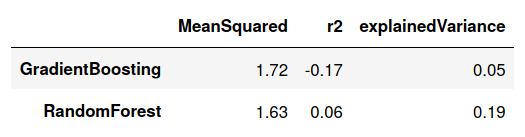
\includegraphics[width=0.6\textwidth]{figure/firstresult}
 	}
 	\caption{Metriken der ersten Modelle}
 	\label{fig:firstresult}
 \end{figure} 
Was bedeuten diese Werte für unsere Modelle?\\
 MeanSquared zeigt den mittleren quadratischen Fehler (MSE) über alle Datenpunkte an. Dieser Wert sag für sich selber nichts über die Güte der Modelle aus, eignet sich aber um verschiedene Modelle miteinander zu vergleichen. Ein niedrigerer Wert ist besser. Ein MSE=0 bedeutet, es gab keinerlei Fehler. Auf der Tabelle sieht man, dass RandomForest besser abgeschnitten hat als GradientBoosting.

Die bestmögliche Punktzahl, die bei $R^2$ erreicht werden kann, ist 1,0. Ein schlechteres Modell erhält einen kleineren Wert. Dieser Wert kann beliebig negativ werden. Ein konstantes Modell, das unter Berücksichtigung der Eingabemerkmale immer den erwarteten Wert von y vorhersagt, würde einen $R^2$-Wert von 0,0 erhalten. Die Werte beider Modelle sind nahe Null und Gradient Boosting sogar negativ. Sonderlich gut vorherzusagen scheinen die Modelle nicht.

Wenn $y$ der Vektor der tatsächlichen Werte ist und $\hat{y}$ die vorhergesagten Werte, dann berechnet $explained\_{}variance(y, \hat{y}) = 1 - \frac{Var\{ y - \hat{y}\}}{Var\{y\}}$ den Wert der Explained-Varianz. Der beste Wert ist 1.0, niedrigere sind schlechter. Üblicherweise sollte ein Modell einen Wert von 0.6 oder höher annehmen, um als valide zu gelten. Davon sind unsere Modelle weit entfernt. Der RandomForest Algorithmus ist minimal besser als GradientBoosting Algorithmus. 

\subsection{Erneut trainieren}
Eine mögliche Ursache für die schlechten Werte könnte sein, dass die Modelle im Training ein niedriges lokales Maxima erreicht haben. Um dies auszuschließen, wiederholen wir das Training auf den selben Daten $n=100$ oft. Abbildung \ref{fig:localminimum}
\begin{figure}[h]
	\centering
	\fbox{	
		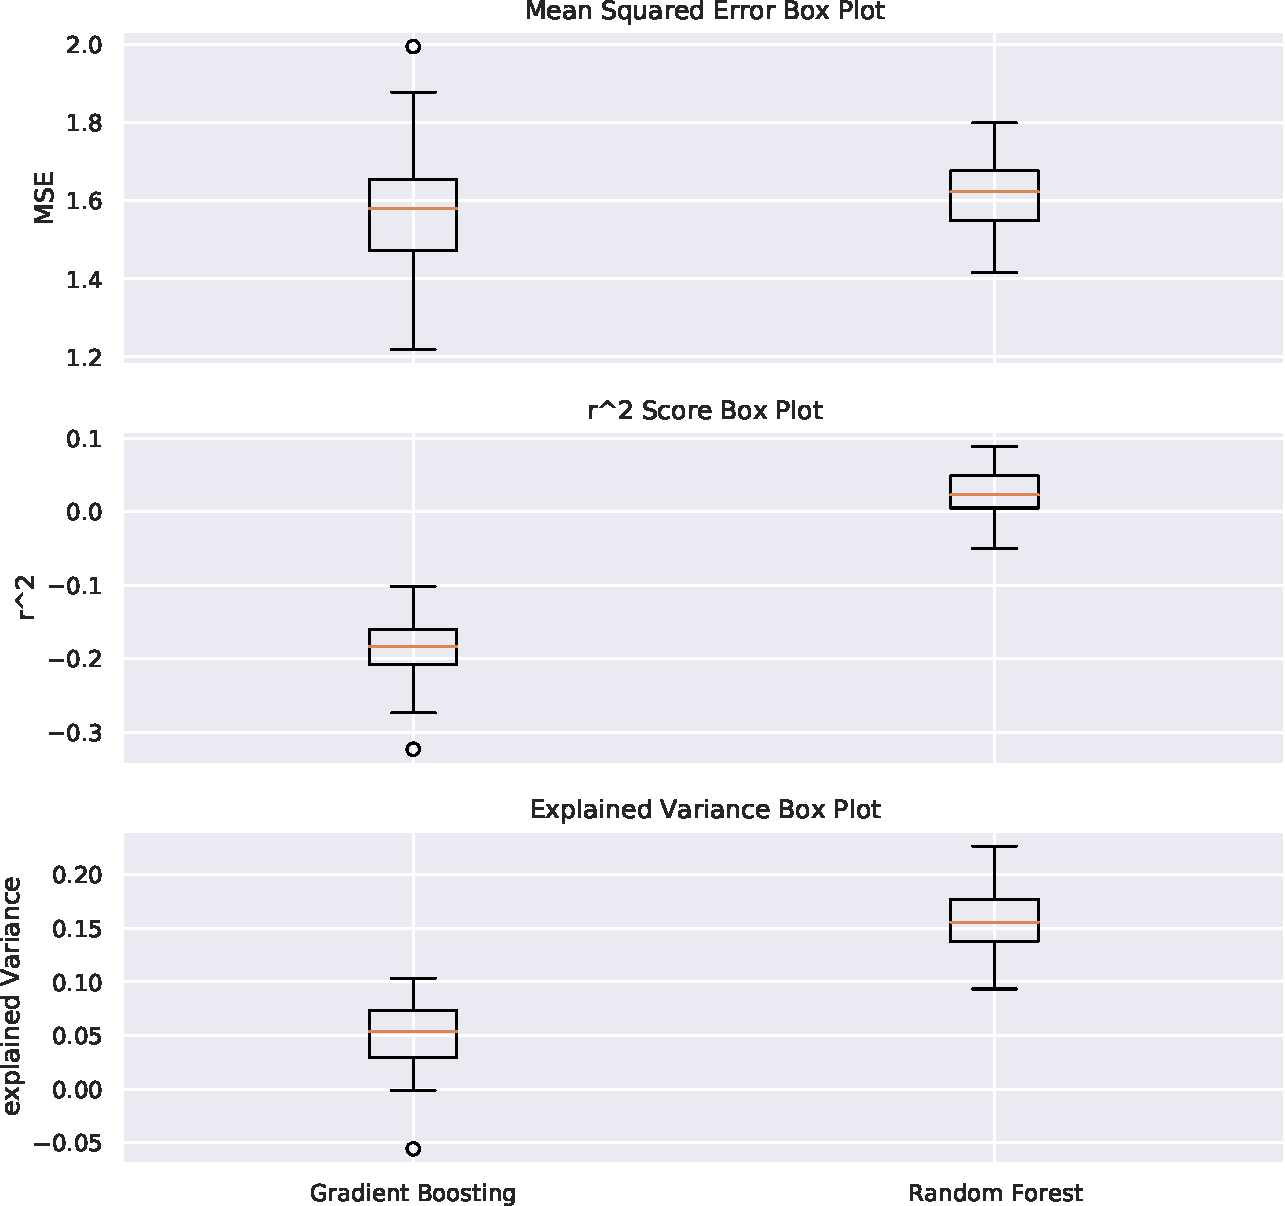
\includegraphics[width=0.6\textwidth]{figure/localminimum}
	}
	\caption{Boxplot der Metriken bei 100 Wiederholungen des Trainings auf den selben Daten}
	\label{fig:localminimum}
\end{figure} 
zeigt das Ergebnis der Auswertung. Auch mit 100 Versuchen erreichten wir keine besseren Werte. Erneut erzielt RandomForest minimal bessere Ergebnisse.
\subsection{Erneut trainieren2}
Eine weitere Quelle für ein schlechtes Ergebnis könnte ein schlechte Wahl der Trainingsdaten sein. Da unsere Menge an Daten nichts sehr groß ist, könnte dies relevant sein. Daher führten wir das Training mehrfach mit zufälligen Trainingsdaten durch und werteten die Modelle aus. Die Methode, die uns diese Arbeit erleichtert ist \href{https://scikit-learn.org/stable/modules/generated/sklearn.model_selection.cross_validate.html}{\lstinline|cross\_validate|}. Das Ergebnis der Cross Validaion ist auf Abbildung \ref{fig:crossval}
\begin{figure}[h]
	\centering
	\fbox{	
		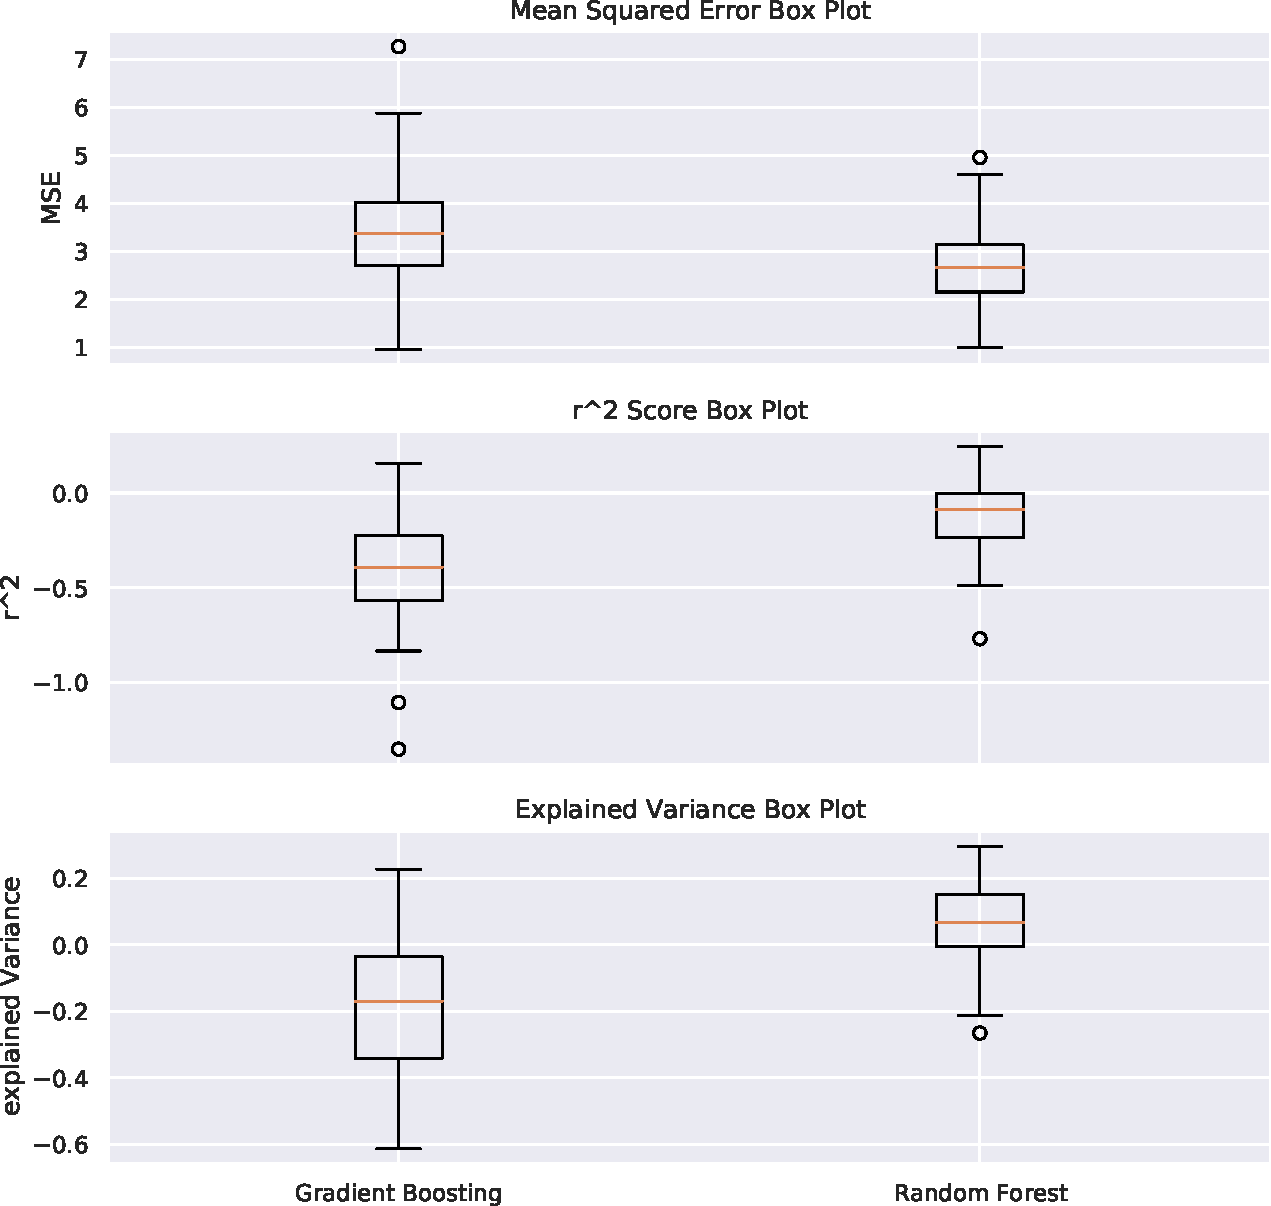
\includegraphics[width=0.6\textwidth]{figure/crossval}
	}
	\caption{Boxplot der Metriken bei 10 Wiederholungen von 5-Fold Cross Validation der Daten}
	\label{fig:crossval}
\end{figure} zu sehen. \\
 Insbesondere an der Verteilung des $R^2$-Scores kann man ablesen, dass beide Modelle in keinem Fall zu wirklich präzise Ergebnissen führen. 
\subsection{Analyse einzelner Parteien}
Insgesamt machten die Modelle keinen guten Eindruck. Das schließt aber nicht aus, dass bei bestimmten Parteien nicht deutliche Tendenzen erkennen zu sind. Wir wiederholten die Tests und analysierten diese für einzelne Parteien. Da uns nicht jede Partei interessierte, untersuchten wir nur die großen Parteien, SPD, CDU, FDP, GRÜNE, DIE LINKE und AFD. Abbildung \ref{fig:simple_parties} \begin{figure}[h]
	\centering
	\fbox{	
		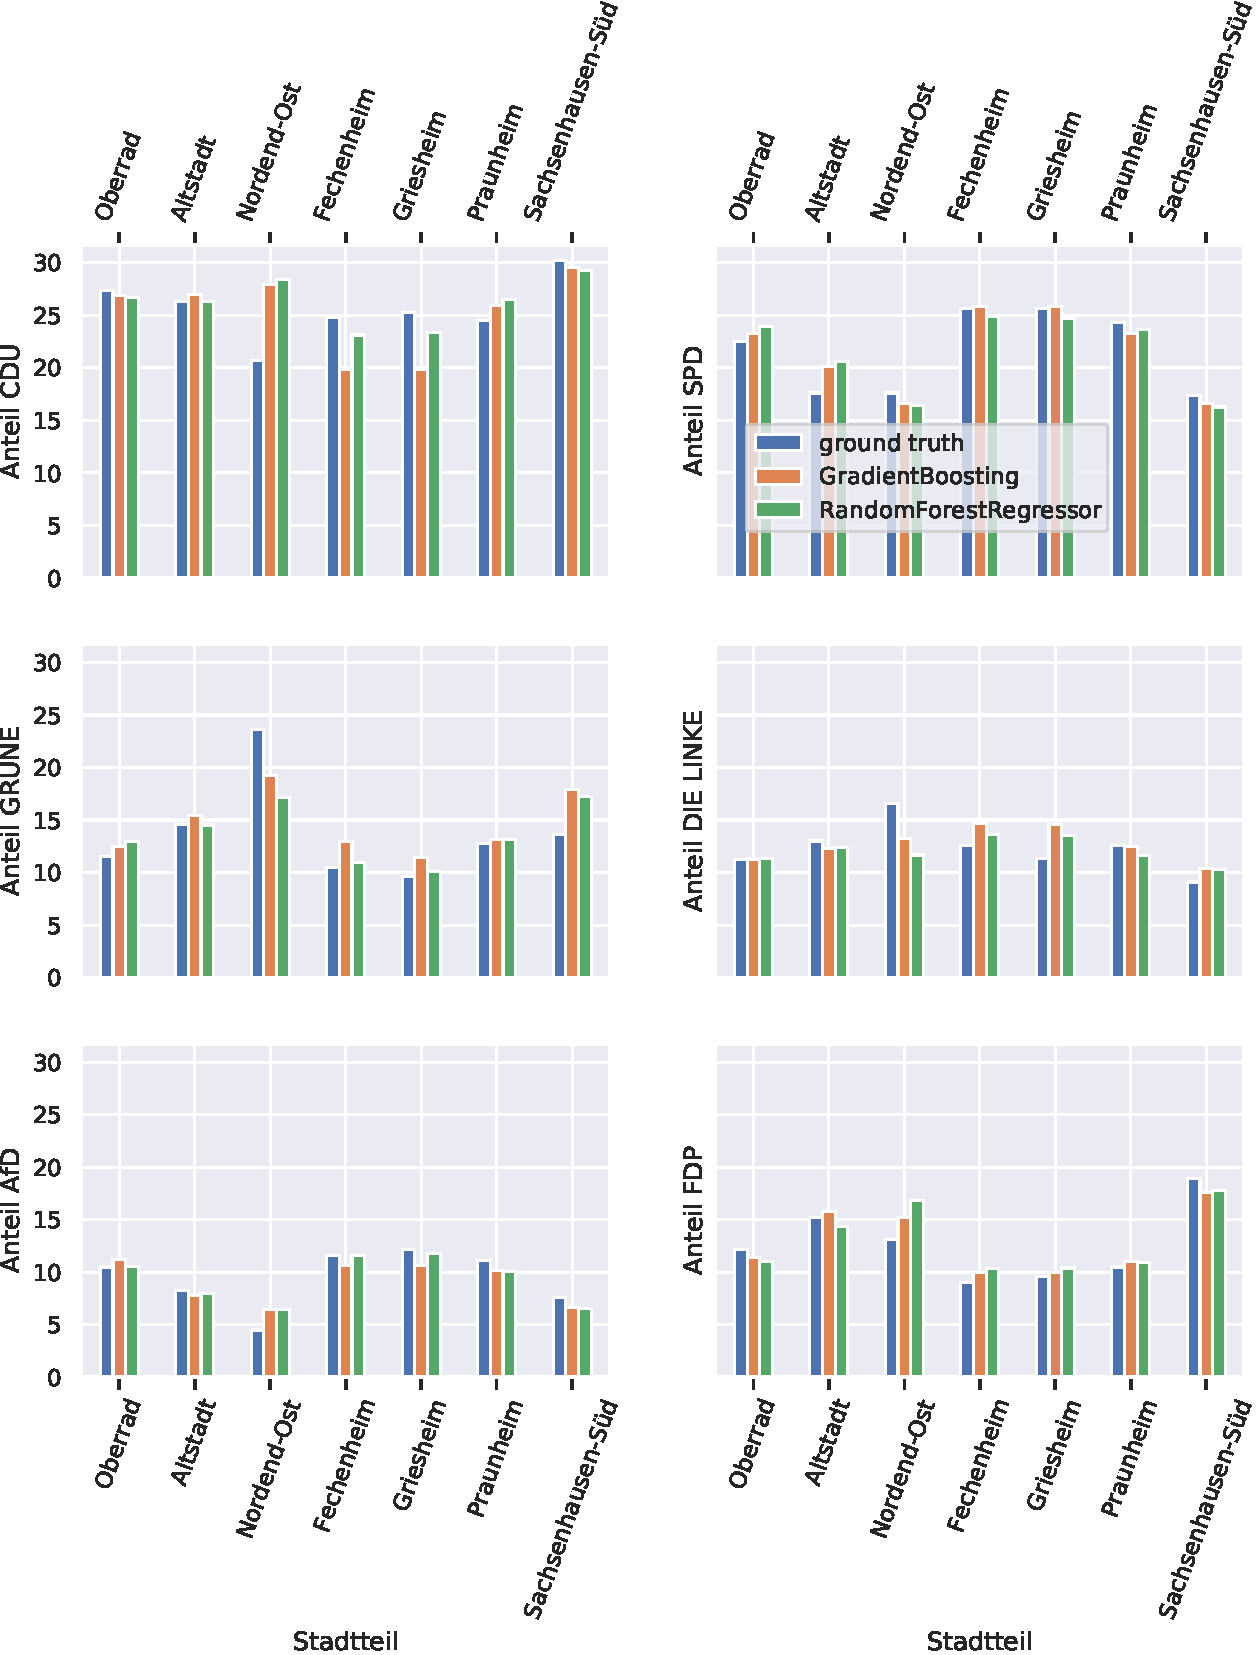
\includegraphics[width=0.9\textwidth]{figure/simple_parties}
	}
	\caption{Vergleich der Vorhersagen zweier Modelle mit der Ground Truth}
	\label{fig:simple_parties}
	\end{figure}  
	zeigt die Vorhersagen unserer beiden ersten Modelle. Man sieht, die Vorhersagen liegen nicht völlig daneben, sie sind nur oft nicht besser als ein konstantes Modell.

 Wir führen die Crossvalidation erneut durch und untersuchen diesmal die einzelnen Parteien. \ref{fig:scores_parties} \begin{figure}
 	\centering
 	\fbox{	
 		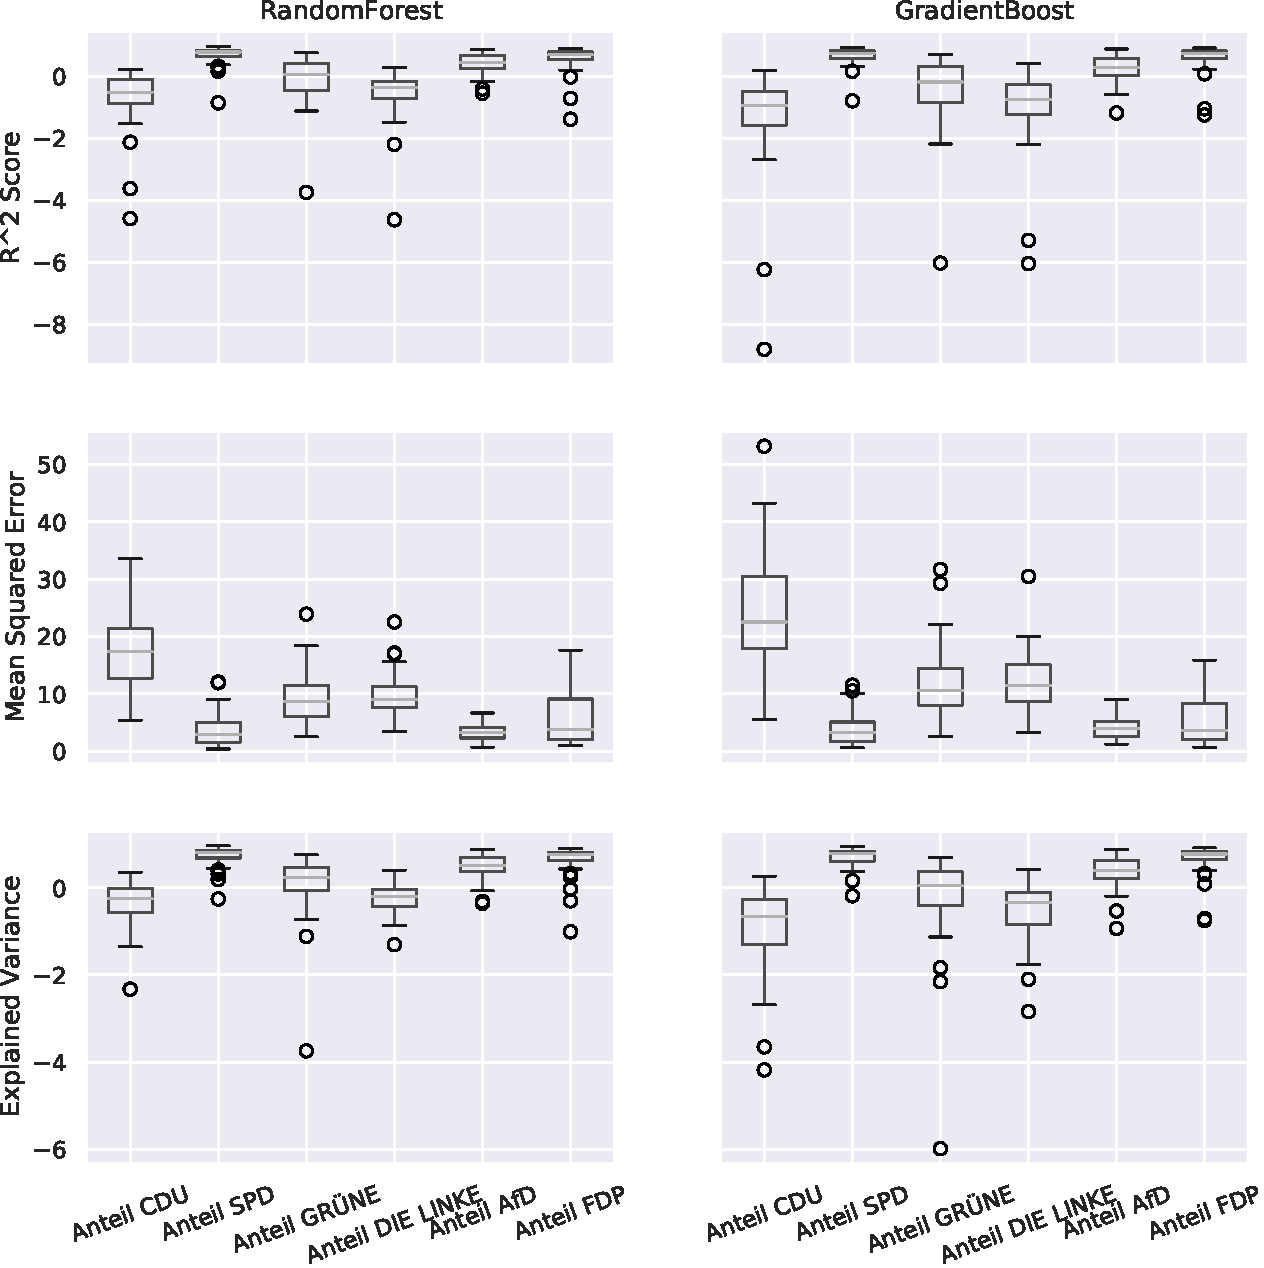
\includegraphics[width=0.9\textwidth]{figure/scores_boxplot_parties}
 	}
 	\caption{Boxplot der Punktzahl verschiedener Metriken der einzelnen Parteien}
 	\label{fig:scores_parties}
 	\end{figure}
 	 Zum einen fällt ins Auge, dass die Varianz der Werte hoch ist. Die Qualität der Modelle hängt also stark von den zufällig ausgewählten Trainingsdaten ab. Die Menge der Trainingsdaten scheint nicht ausreichend, um ein gutes  Modell zu erstellen. \\
Andererseits sehen wir drei Parteien: SPD, DIE LINKE und AFD, für die im Schnitt die Modelle deutlich besser als ein vergleichbares konstantes Modell sind. Dies können wir daran ablesen, dass dort der $R^2$-Score und die Explained Varianz meist über 0 sind. Gleichzeitig ist für diese Parteien der Mean Squared Error deutlich niedriger als für den Rest der Parteien. 
 


\section{Konklusion}
Es scheint, dass zumindest mit den von uns verwendeten Einkommensdaten und den verwendeten Modellen eine generelle Prognose des Wahlverhaltens eines Stadtteils in Frankfurt nicht möglich ist. Kritisch an den von uns verwendeten Daten ist sicherlich die zeitliche Differenz der beiden Datensätze und die Korrelation der Eingabe und die Korrelation der Ausgabe Werte untereinander, da die von uns verwendeten ML Algorithmen von unabhängigen Parametern ausgehen.\\
 Der Unterschied in beiden Algorithmen ist minimal mit kaum erwähnenswerten Vorteilen für RandomForestRegressor. Vermutlich variieren die von GradientBoostingRegressor gesuchten Maxima zu sehr während RandomForestRegressor etwas davon profitiert, dass er auch Korrelation zwischen Klassen erkennt.  \\
 Für uns überraschend jedoch ist das Ergebnis, das selbst trotz der eben beschrieben Mängel unser trainiertes Modell für die Parteien DIE LINKE, SPD und AFD erstaunlich bessere Werte liefert als für CDU, FDP und DIE GRÜNEN. Diese legt die Vermutung nahe, dass zumindest für das Ergebnis der ersten drei Parteien die Einkommensverteilung in einem Stadtviertel eine größere Rolle spielt als für letztere.\\
Selbstverständlich war nicht zu erwarten, dass ein so komplexer Prozess wie das Wahlverhalten eines Stadtviertels sich nur von der Einkommensverteilung des Stadtviertels vorhersagen lässt. Es spielen sicherlich aktuelle Geschehnisse, langjährige Parteienbindung und viele andere schwer messbare Faktoren eine entscheidendere Rolle. Doch für das Ergebnis einige Parteien hier in Frankfurt scheint die Einkommensverteilung der Wähler eine gewisse Relevanz zu besitzen. 
\end{document}
